%
% federpendel.tex
%
% (c) 2025 Prof Dr Andreas Müller
%
\documentclass[tikz]{standalone}
\usepackage{amsmath}
\usepackage{times}
\usepackage{txfonts}
\usepackage{pgfplots}
\usepackage{csvsimple}
\usetikzlibrary{arrows,intersections,math}
\begin{document}

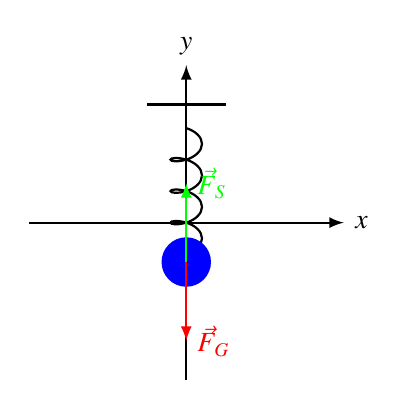
\begin{tikzpicture}[>=latex,thick]
    % Koordinatensystem
    \draw[->] (-2,0) -- (2,0) node[right] {$x$};
    \draw[->] (0,-2) -- (0,2) node[above] {$y$};
    
    % Feder
    \draw[thick] (0,1.5) -- (0,1.2);
    \draw[thick, decorate, decoration={coil, aspect=0.5, segment length=4mm, amplitude=2mm}] (0,1.2) -- (0,-0.5);
    
    % Körper
    \filldraw[blue] (0,-0.5) circle (0.3) node[below] {$m$};
    
    % Kräfte
    \draw[->, thick, red] (0,-0.5) -- (0,-1.5) node[right] {$\vec{F}_G$};
    \draw[->, thick, green] (0,-0.5) -- (0,0.5) node[right] {$\vec{F}_S$};
    
    % Aufhängung
    \draw[thick] (-0.5,1.5) -- (0.5,1.5);
\end{tikzpicture}

\end{document}
